%-*- mode: LaTex; outline-regexp: "\\\\section\\|\\\\subsection";fill-column: 80; -*-
\documentclass[12pt]{article}
\usepackage[longnamesfirst]{natbib}
\usepackage[usenames]{color}
\usepackage{graphicx}  % Macintosh pdf files for figures
\usepackage{amssymb}   % Real number symbol {\Bbb R}
\usepackage{bbm}
\input{../../standard}

% --- margins
\usepackage{../sty/simplemargins}
\setleftmargin{1in}   % 1 inch is NSF legal minimum
\setrightmargin{1in}  % 1 inch is NSF legal minimum
\settopmargin{1in}    % 1 inch is NSF legal minimum
\setbottommargin{1in} % 1 inch is NSF legal minimum

% --- Paragraph split, indents
\setlength{\parskip}{0.20in}
\setlength{\parindent}{0.20in}

% --- Line spacing
\renewcommand{\baselinestretch}{1.5}

% --- page numbers
\pagestyle{empty}  % so no page numbers

% --- Hypthenation
\sloppy  % fewer hyphenated
\hyphenation{stan-dard}
\hyphenation{among}

% --- Customized commands, abbreviations
\newcommand{\TIT}{{\it  {\tiny Leverage and Model Selection (\today)}}}

% --- Header
\pagestyle{myheadings}
\markright{\TIT}

% --- Title

\title{ Leveraged Outliers and Model Selection }
\date{\today}

%%%%%%%%%%%%%%%%%%%%%%%%%%%%%%%%%%%%%%%

\begin{document}
% \maketitle 


%--------------------------------------------------------------------------
\section{ To Do }
%--------------------------------------------------------------------------

 Link back to earlier work in finding that CVSS and AIC were not pointing for us
 to pick the same model.


%--------------------------------------------------------------------------
\section{ Motivation }
\label{sec:motivation}
%--------------------------------------------------------------------------

 Problem is motivated by selecting features for a regression using features
 derived from the singular value decomposition of the document/term matrix of
 text documents.  The response is a property associated with a document (in our
 case, the price of a house described by a listing) and the features are
 eigenwords from the text of a collection of listings.  Rather than try to find
 the best subset, the monotone nature of the predictive value of these features
 suggests picking in order, much like one does with an autoregression (albeit on
 a larger scale).  Should we use the first 10, 30, or 50 singular vectors (\ie,
 eigenwords) as features?  The problem is complicated by the presence of
 outliers produced by the decomposition.  Given the Ziphian distribution
 associated with text, outliers are to be expected.


 More generally, leveraged observations produce surprising effects on regression
 models, particularly by producing collinearity among the explanatory features.
  Leveraged observations in our setting are simply rows of the design matrix $X$
 that have large variance compared to typical rows.


%--------------------------------------------------------------------------
\section{ Stylized Problem }
\label{sec:problem}
%--------------------------------------------------------------------------

 The following example illustrates what can happen.  For this example, we
 simulated $n = 1000$ observations $X_i = (X_{i1},\ldots,X_{ip})'$ of $p = 100$
 independent Gaussian variables.  The first $n_o$ obsevations have variance
 $\sigma_o^2$, and the remaining observations have variance 1.  otherwise.
 \begin{equation}
    X_{ij} \sim \left\{ \begin{array}{cc}
              N(0,\sigma_o^2), & i \le n_o \cr
              N(0,1)    , & n_o < i \le n \;.
   \end{array} \right.
 \label{eq:Xij}
 \end{equation}
 These first 50 cases are the leveraged observations; the observations are
 independent, but not identically distributed.  The model for the response is
the usual Gaussian regression with {\em constant} error variance,
 \begin{equation}
   Y_i = \beta_0 + \beta_1 X_{i1} + \cdots + \beta_p X_{ip} + \sigma \ep_i,
        \quad \ep_i \sim N(0,1) \;.   
 \label{eq:Yi}
 \end{equation}
 Notice that the model is {\em not} heteroscedastic; rather, the changing
variances occur among the values of the $X_{ij}$.


 Now suppose that we know that only the first $k$ elements of $\beta$ are
 non-zero.  How should we pick the best fitting regression, that minimizes the
 squared error of prediction?  As will become clear, this question is not well
 posed.  A popular choice for this context is to use \aic, which we illustrate
 in a small simulation.  Suppose $n = 2000$ with $p = 150$, with $n_o=50$
 leverage points with $\sigma_o = 100$.  Before continuing, we note that the
 presence of these leverage points produces a surprising amount of collinearity
 given that the design points are independent.  Figure \ref{fig:cn} graphs the
 condition number of the leading columns of the design matrix, varying the
 number of columns included.  (The condition number is the ratio of the largest
 to smallest singular value of a non-square matrix.) The left frame shows the
 condition number if $\sigma_o = 1$ (\ie, without leverage points); the
 condition number grows roughly linearly in the number of columns (slope
 $\approx 0.0046$).  The right frame of Figure \ref{fig:cn} shows the condition
 number in the context of our simulated data with $n_o = 50$ and $\sigma_o =
 100$.  Again, the condition number increases linearly, but with a much steeper
 slope near 0.26.  But for the scale of the y-axis, the figures are almost
 identical.  Notice that the linear growth persists for matrices with more than
 $n_o$ columns; larger matrices do not quickly ``outgrow'' the influence of the
 leverage points.  The amount of collinearity grows at a steady fixed rate (for
these dimensions) as the number of columns increases.

 \begin{figure}
 \caption{ Condition numbers for matrices with increasing numbers of columns,
 with with no leveraged outliers (left) or with $n_o=50$ leveraged outliers with
 standard deviation $\sigma_o=100$ (right). } 
 \label{fig:cn}
 \centerline{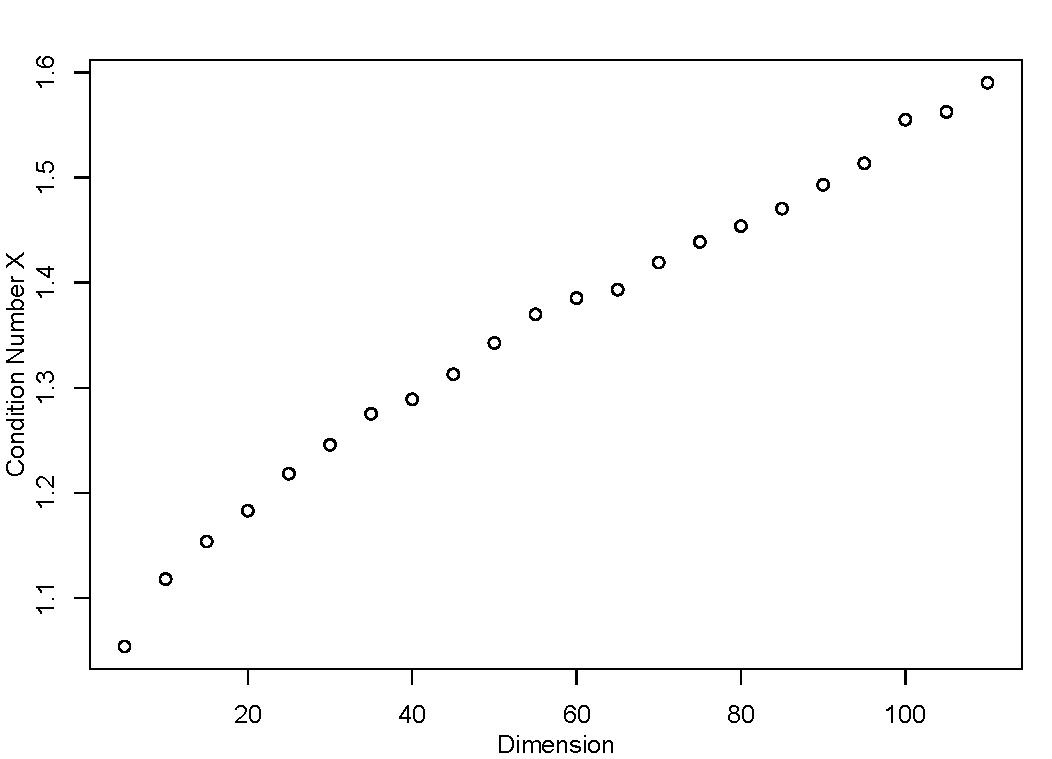
\includegraphics[width=2.5in]{figures/cn1.pdf}
             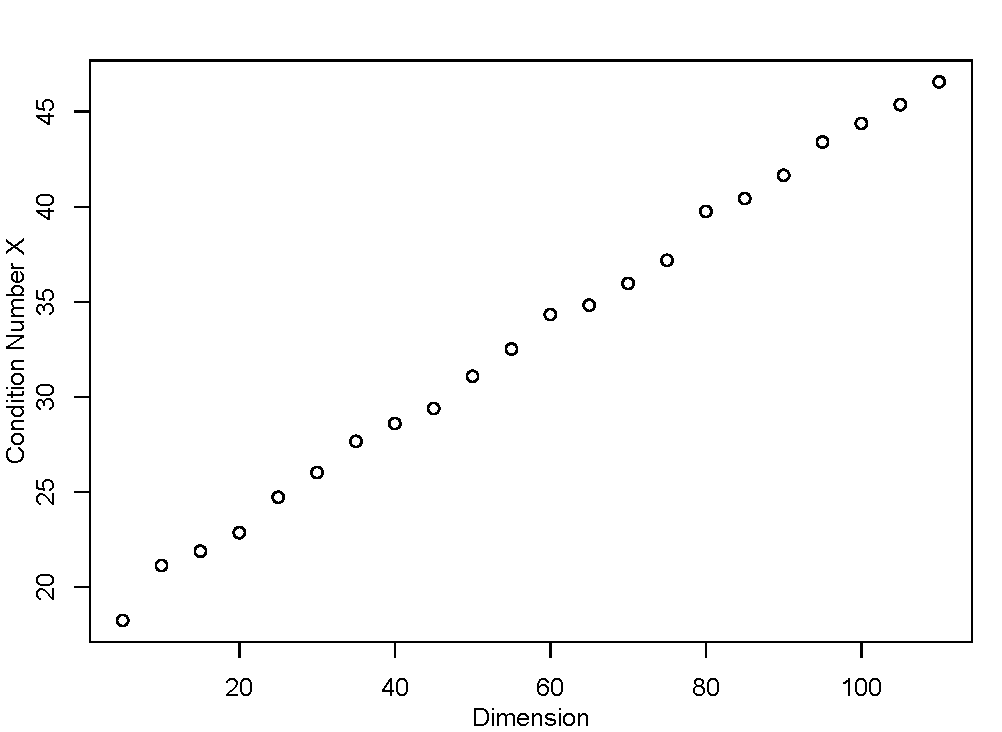
\includegraphics[width=2.5in]{figures/cn100.pdf}}
 \end{figure}


 Figure \ref{fig:example1} shows the impact of this colllinearity on the problem
 of picking a model. For this illustration, $k = 75$ features are predictive.
  We set $\beta_j = c$ for $j = 1,\ldots,k$ with $c$ chosen so that these
 coefficients lie, on average about 5 standard errors from 0.  These are very
 significant effects, and $R^2 \approx 0.53$ for the fully specified model with
 all 75 features.  The top frame of Figure \ref{fig:example1} plots of two forms
 of \aic\ for models of increasing size.  The White version of \aic\ uses a
 heteroscedastic consistent variance estimate rather than the fitted
 estimate. (We also use the estimate of $\sigma^2$ from the prior model when
 computing \aic.) The version of \aic\ corrected for heteroscedasticity shows a
 dramatic valley and relatively steep increase past its minimum.  Though showing
 different trends, the two versions of \aic\ both pick a model with about 50
 features, substantially fewer than $k=75$ and matching the number of leverage
 points.  In both panels of Figure \ref{fig:example1}, we have normalized the
 statistics to lie on a common range for visual comparisons.  The vertical gray
 line in this and other figures highlights the number of leveraged outliers in
 the data (in this case, $n_o=50$).  Other colored colored segments denote the
 position of the minimum value.

 \begin{figure}
 \caption{ Simulation of \aic\ (normal in blue and heteroscedastic consistent,
 top) and model loss and mean squared prediction errors (bottom), in the
 presence of leverage points.  The loss is shown in black, with the
 ``in-sample'' error $\normsq{X_{1:j}(\hat\beta_{1:j}-\beta_{1:j}}$ and the
 corresponding ``out-of-sample'' error when the estimates are applied to new
 observations. }
 \label{fig:example1}
  \centerline{ 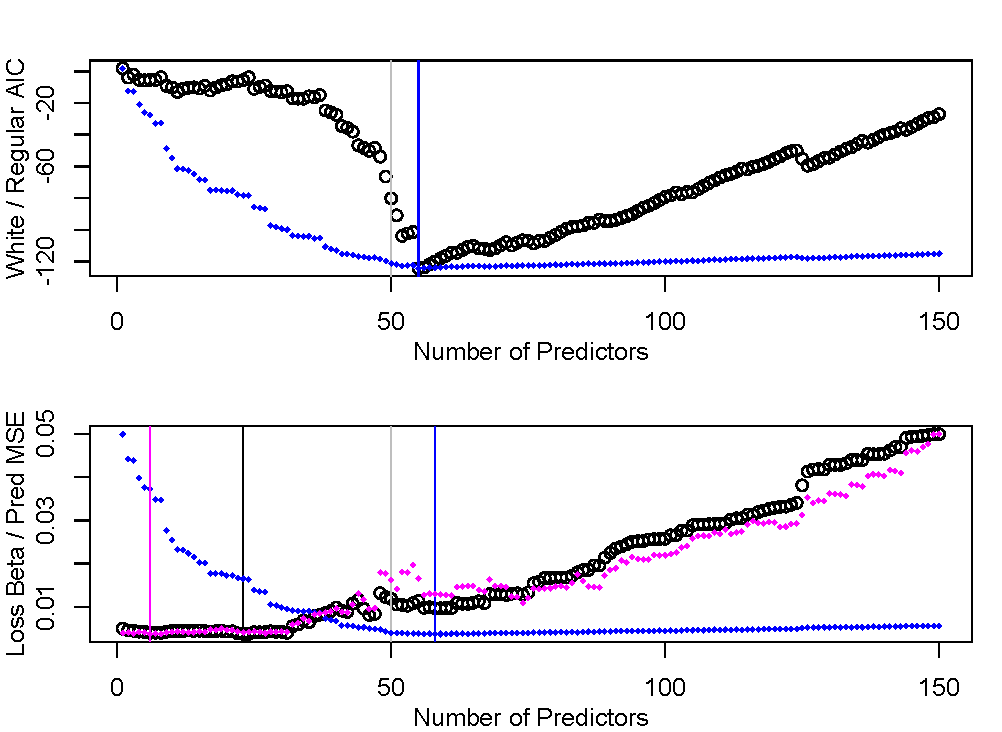
\includegraphics[width=5in]{figures/example1.pdf} }
 \end{figure}

 The lower panel shows how well these models perform. Whereas both versions of
 \aic\ are computable; the lower panel shows unobservable errors that are
 computable only because we have simulated these data from known
 populations. The black points in the figure show the model loss.  Let $X_{0:j}$
 refer to a matrix comprised of a column of 1's followed by the first $j$
 columns of $X$, and similarly let $\beta_{0:j}$ and $\hat\beta_{0:j}$ refer to
 the associated true coefficients and least squares estimates (including the
 intercept).  The model loss (black points) is then the sequence 
 \begin{displaymath}
    \normsq{ \beta_{0:j} - \hat\beta_{0:j}} \;, \quad j = 1,\ldots,150 \;.
 \end{displaymath}
 The sequence of blue points in the figure are the ``in-sample'' mean squared
errors, computed as 
 \begin{displaymath}
    \mbox{In-Sample MSE:  } \normsq{ X_{0:j}(\hat\beta_{0:j}-\beta_{0:j}) }   
 \end{displaymath} 
 This sequence is highly correlated with the trend of the usual \aic\ statistic
 in the upper panel.  The ``out-of-sample'' version of the mean squared error is
 computed by drawing a second realization of the design matrix from the same
 process (and the same choices for simulating leverage points), independently,
 and computing the prediction error for these features.  With this independent
realization of $X$ labeled $\widetilde{X}$, the magenta points in the lower
panel of Figure \ref{fig:example1} show
 \begin{displaymath}
    \mbox{Out-of-Sample MSE:  } \normsq{ \widetilde{X}_{0:j}(\hat\beta_{0:j}-\beta_{0:j}) }   
 \end{displaymath} 
 This version of the mean squared error closely mimics the trend in the loss,
 which after all is its expectation (over the distribution of $X$).


 In the presence of leverage points, \aic\ thus tries to pick a model that
 predicts {\em the observed} cases well.  After all, that's the only data
 visible.  What we more often experience in practice, however, is the behavior
 seen of the out-of-sample MSE.  Thus, \aic\ is solving one problem (evidently
 pretty well), but it may not be the problem we care about.  Without the
 leverage points (and the collinearity they induce), the issues raised here
 vanish.  Figure \ref{fig:example2} shows the same statistics and random
 variables as Figure \ref{fig:example1}, but wihout the leverage points. Both
 versions of \aic\ align closely and pick the correct model with $k=75$
 features, and all of the error measures agree.

 \begin{figure}
 \caption{ Simulation of \aic\ (normal in blue and heteroscedastic consistent,
 top) and model loss and mean squared prediction errors (bottom), without
leverage points. }
 \label{fig:example2}
  \centerline{ 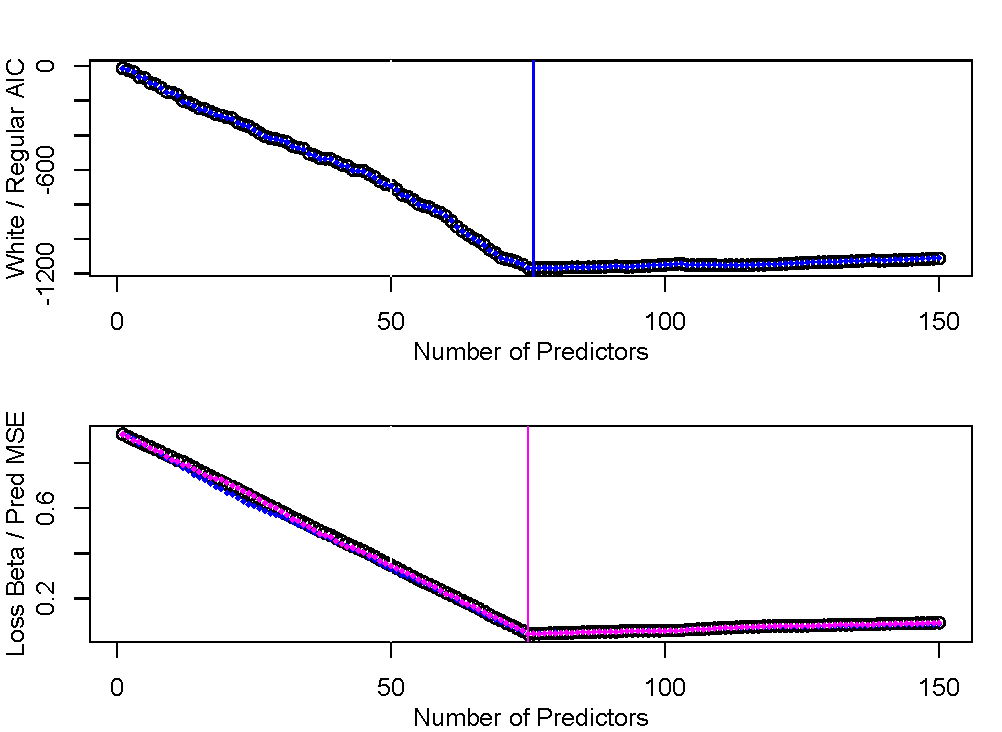
\includegraphics[width=5in]{figures/example2.pdf} }
 \end{figure}



%--------------------------------------------------------------------------
\section{ xx }
\label{sec:}
%--------------------------------------------------------------------------


%--------------------------------------------------------------------------
\section{ xx }
\label{sec:}
%--------------------------------------------------------------------------



%--------------------------------------------------------------------------
\section{ Derivations  }
\label{sec:derive}
%--------------------------------------------------------------------------


%--------------------------------------------------------------------------
% References
%--------------------------------------------------------------------------

\bibliography{../../../references/stat,../../../references/TextPapers/text}
\bibliographystyle{../bst/ims}

\end{document} %==========================================================
